\documentclass{article}

%%%% PAGE FORMATTING %%%%
\usepackage[margin=1in, includefoot]{geometry}
\usepackage{fancyhdr}
\pagestyle{fancy}
\fancyhead{}
\fancyfoot{}
\fancyfoot[R]{ \thepage\ }
\renewcommand{\footrulewidth}{1pt}
\renewcommand{\headrulewidth}{1pt}
\setlength{\parindent}{0pt}


%%%% FONTS %%%%
\usepackage[T1]{fontenc}
\usepackage[sfdefault]{AlegreyaSans} % sfdefault makes sans serif default.
\renewcommand*\oldstylenums[1]{{\AlegreyaSansOsF #1}}
\usepackage[usenames, dvipsnames]{color}


%%%% LISTS %%%%
\usepackage{enumitem}


%%%% TABLES %%%%
\usepackage{tabularx}
\usepackage{caption}
\captionsetup[table]{skip=10pt}
\newcolumntype{P}[1]{>{\centering\arraybackslash}p{#1}}
\setlength{\tabcolsep}{20pt}
\renewcommand{\arraystretch}{1}


%%%% FIGURES %%%%
\usepackage{graphicx}
\usepackage{float}


%%%% TIKZ PICTURES %%%%
\usepackage{tikz}
\usetikzlibrary{shapes}
\usetikzlibrary{positioning}
\usetikzlibrary{patterns}
\usepackage{pgf}
\usetikzlibrary{arrows.meta,bending}
\usetikzlibrary{decorations.pathmorphing}
\usetikzlibrary{decorations.markings}


%%%% MATHEMATICS %%%%
\usepackage{amsmath}
\usepackage{amsthm}
\usepackage{amssymb}
\usepackage{mathtools} % For prescripts.
\renewcommand{\vec}[1]{\textbf{#1}} % Vectors appear as boldface.
\usepackage{braket} % For braket notation.
\usepackage{tensor} % For tensor indices.


%%%% FRAMED MATHEMATICS ENVIRONMENTS %%%%
\usepackage{framed}

\newcounter{framedmath}[section]
\newenvironment{framethm}[1][]{\refstepcounter{framedmath} \begin{framed} \noindent \textbf{Theorem~\thesection.\theframedmath:} #1}{\end{framed}} 

\newenvironment{framethmstar}[1][]{\refstepcounter{framedmath} \begin{framed} \noindent \textbf{*Theorem~\thesection.\theframedmath:*} #1}{\end{framed}} 

\newenvironment{framelem}[1][]{\refstepcounter{framedmath} \begin{framed} \noindent \textbf{Lemma~\thesection.\theframedmath:} #1}{\end{framed}} 

\newenvironment{framecor}[1][]{\refstepcounter{framedmath} \begin{framed} \noindent \textbf{Corollary~\thesection.\theframedmath:} #1}{\end{framed}} 
   
\newenvironment{frameex}[1][]{\refstepcounter{framedmath} \begin{framed} \noindent \textbf{Example~\thesection.\theframedmath:} #1}{\end{framed}} 

\newenvironment{framedef}[1][]{\refstepcounter{framedmath} \begin{framed} \noindent \textbf{Definition~\thesection.\theframedmath:} #1}{\end{framed}} 

\newenvironment{frameax}[1][]{\refstepcounter{framedmath} \begin{framed} \noindent \textbf{Axiom~\thesection.\theframedmath:} #1}{\end{framed}} 

\newenvironment{frameprop}[1][]{\refstepcounter{framedmath} \begin{framed} \noindent \textbf{Proposition~\thesection.\theframedmath:} #1}{\end{framed}} 

%%%% MARGIN NOTES %%%%
\usepackage[fulladjust]{marginnote}

\makeatletter
\renewcommand\marginfont{\normalfont}
\renewcommand\raggedleftmarginnote{\@parboxrestore\@marginparreset\raggedleft}
\renewcommand\raggedrightmarginnote{\@parboxrestore\@marginparreset\raggedright}
\makeatother

\newcounter{lecture}
\newcommand{\lecture}{\refstepcounter{lecture}\reversemarginpar\marginnote{\ding{70} \textit{Lecture ~\thelecture}}}


%%%% FUN SYMBOLS %%%%
\usepackage{pifont}


%%%% PAGE RULES %%%%
\newcommand{\minirule}{\begin{center}\rule{0.7\textwidth}{.4pt}\end{center}}


%%%% CONTENTS LINES %%%%
\newcommand{\describesection}[1]{\addtocontents{toc}{\textit{\footnotesize \hspace{37pt} #1}\par\vspace{0.1cm}}}


%%%% HYPERLINKS %%%%
\usepackage{hyperref}
\hypersetup{
    colorlinks=true,
    linkcolor=red,
    filecolor=black,      
    urlcolor=red,
}


%%%% CODE %%%%
\usepackage{listings}
\usepackage{color}

\DeclareFixedFont{\ttb}{T1}{txtt}{bx}{n}{8} % for bold
\DeclareFixedFont{\ttm}{T1}{txtt}{m}{n}{8}  % for normal

\definecolor{deepblue}{rgb}{0,0,0.5}
\definecolor{deepred}{rgb}{0.6,0,0}
\definecolor{deepgreen}{rgb}{0,0.5,0}

\newcommand\pythonstyle{\lstset{
language=Python,
basicstyle=\ttm,
morekeywords={self},              % Add keywords here
keywordstyle=\ttb\color{deepblue},
emph={MyClass,__init__},          % Custom highlighting
emphstyle=\ttb\color{deepred},    % Custom highlighting style
stringstyle=\color{deepgreen},
frame=tb,                         % Any extra options here
showstringspaces=false,
numbers=left,
numberstyle=\small\color{gray}
}}

\lstnewenvironment{python}[1][]
{
\pythonstyle
\lstset{#1}
}
{}


%%%% FLAG ERROR IN NOTES %%%% 
\newcommand{\flag}[1]{{\color{red} #1}}


\begin{document}

%%%% TITLE, AUTHORS AND TABLE OF CONTENTS %%%%
\title{\textbf{Machine Learning for High Energy Physics}}
\date{}
\author{\textit{Notes taken by Manuel Morales \& James Moore}\\ \textit{at the MLHEP summer school}}
\maketitle

\renewcommand*\contentsname{}
\tableofcontents


%%%% INTRODUCTION %%%%
\newpage
\part{Introduction to machine learning}
\hrule
\noindent \\
\section{Introduction to supervised learning}

\subsection{Problem setup}
\describesection{Problem setup for supervised learning. Basic examples.}

\begin{framedef}
Consider a set $\mathcal{X}$ of objects and a set of targets $\mathcal{Y}$. Suppose also that there is an unknown function $f : \mathcal{X} \rightarrow \mathcal{Y}$ mapping objects into targets (which may be stochastic - by which we mean the objects and targets are drawn from some joint probability distribution).\\

A \textit{dataset} is a finite collection $D = \{(x_i,f(x_i)) : i=1,...,N\} \subseteq \mathcal{X} \times \mathcal{Y}$. The goal of \textit{supervised learning} is to \textit{approximate $f$ given a dataset $D$} (i.e. learn to recover targets from objects). 
\end{framedef}

\begin{frameex}
\begin{enumerate}[label = (\roman*)]
\item \textbf{Classification of iris flower species.} The objects $\mathcal{X}$ are individual flowers, described by the length and width of their sepals and petals. The targets $\mathcal{Y}$ are the species to which the flowers belong. The mapping $f : \mathcal{X} \rightarrow \mathcal{Y}$ takes a flower to its species (and depends on different shapes of sepals, petals, etc corresponding to the different species). Note this is a \textit{non-deterministic} mapping because the growth of a certain flower is associated with a number of random processes.
\item \textbf{Spam filtering.} The objects $\mathcal{X}$ are emails (sequences of characters). The targets are the categories $\mathcal{Y} = \{\text{spam}, \text{not spam}\}$. The mapping $f : \mathcal{X} \rightarrow \mathcal{Y}$ tells us whether a particular email $x \in \mathcal{X}$ is spam or not, and is again \textit{non-deterministic} (the style and content can vary from author to author).
\item \textbf{CAPTCHA recognition.} The set of objects $\mathcal{X}$ is a set of CAPTCHA images (which are really vectors of pixel level brightness). The set of targets $\mathcal{Y}$ are sequences of characters, relating to the correct word that the CAPTCHA shows. The mapping $f : \mathcal{X} \rightarrow \mathcal{Y}$ is the inverse of the algorithm used to generate the CAPTCHA - this is \textit{almost} deterministic, but depends on the level of distortion (very high distortion can make the map less deterministic).
\item \textbf{Particle identification in a HEP experiment.} The objects $\mathcal{X}$ are particles, described by the detector experiments (e.g. track parameters, calorimeter energy, deposit, etc.). The targets $\mathcal{Y}$ are the types of the particles (e.g. electrons, muons, protons, etc.). The mapping $f : \mathcal{X} \rightarrow \mathcal{Y}$ is the inverse of the physical process generating the detector response (by definition, this is a stochastic process).
\end{enumerate}
\end{frameex}



\newpage
\subsection{Feature types}
\describesection{Features and the design matrix. Numeric, categorical nominal, categorical ordinal and binary features. One-hot encoding.}
Typically the objects in our set $\mathcal{X}$ will have some structure.

\begin{framedef}
Let $\mathcal{X}$, $\mathcal{Y}$ be the sets of objects and targets in a supervised learning problem. Suppose that $\mathcal{X}$ is a collection of \textit{tuples}, so that given a dataset $D \subseteq \mathcal{X} \times \mathcal{Y}$, for each $(x_i,f(x_i)) \in D$ we can write $x_i$ as:
\begin{equation*}
x_i = (x_i^1,x_i^2,...,x_i^d),
\end{equation*}
for some $d$ (which need not be the same for all $x_i \in \mathcal{X}$). We say that $x_i^j$ is a \textit{feature} of the object $x_i$ (note we use the upper index for the \textit{feature}, and the lower index to label the object in the dataset).\\

Many algorithms require that the \textit{dimensionality} $d$ of the data is the same for all objects. In this case, the dataset can be represented by a \textit{design matrix}:
\begin{equation*}
X = \begin{pmatrix} x_1^1 & x_1^2 & \cdots & x_1^d \\ x_2^1 & x_2^2 & \cdots & x_2^d \\ \vdots & \vdots & \ddots & \vdots \\ x_N^1 & x_N^2 & \cdots & x_N^d \end{pmatrix}.
\end{equation*}
The column index corresponds to the features, and the row index corresponds to the position of the object in the dataset.
\end{framedef}

\begin{frameex}
Consider the problem of classifying species of irises. In this case, features might include \textit{sepal length}, \textit{sepal width}, \textit{petal length} and \textit{petal width}. In this case, all of the features are real numbers.\\

Since each flower will have these features, we can describe all objects as $4$-tuples, and hence we can organise the data into a $N \times 4$ design matrix.
\end{frameex}


\begin{framedef}
In general, features $x_i^j$ might be of varying natures. We give special names to some common cases:
\begin{itemize}
\item \textit{Numeric features} take values in (for example) the real numbers. For example sepal length in the classification of iris species, building height, or particle transverse mometnum.
\item \textit{Categorical nominal features} take values in a finite set, with no natural ordering. For example colour, city of birth or particle type.
\item \textit{Categorical ordinal features} take values in a set equipped with a natural order, for example level of education, age, or particles passing loose, medium or tight selection criteria.
\item \textit{Binary features} take values in a set of size $2$, for example $\{\text{true}, \text{false}\}$, $\{0,1\}$, $\{-1,+1\}$. 
\end{itemize}
\end{framedef}

A natural question that arises in the handling of data is how one might convert a categorical nominal feature into a binary or numeric feature (since binary or numeric features can be more easily handled).\\

A na\"{i}ve approach would be to assign each category a number (e.g. red$=1$, green$=2$, etc). However, this introduces an ordering on the feature, which could have a negative effect on learning algorithms later on. 


\newpage
A better solution is \textit{one-hot encoding}:

\begin{framedef}
Let $x_i = (x_i^1,...,x_i^{j-1},x_i^j,x_i^{j+1}, ..., x_i^d)$ be an object in a dataset, and let $x_i^j$ be a categorical nominal feature for the object, taking values in some finite set $S$. A \textit{one-hot encoding} replaces the feature $x_i^j$ with $|S|$ binary features $\{x_i^{j,s} : s \in S\}$ obeying:
\begin{equation*}
x_i^{j,s} = \begin{cases} 0 & \text{if $x_i^j \neq s$,}\\ 1 & \text{if $x_i^j = s$.} \end{cases}
\end{equation*}
The new object then takes the form 
\begin{equation*}
x_i = (x_i^1,...,x_i^{j-1}, x_i^{j,s_1},...,x_i^{j, s_{|S|}}, x^{j+1},...,x_i^d),
\end{equation*}
where $s_i \in S$ are the elements of $S$.
\end{framedef}

\begin{frameex}
Suppose $x$ is a categorical nominal feature taking values in the set $\{\text{red}, \text{blue}, \text{green}\}$. A one-hot encoding of the object is:
\begin{equation*}
(x^{\text{red}}, x^{\text{blue}}, x^{\text{green}}),
\end{equation*}
where $x^{\text{red}} = 0$ if $x \neq \text{red}$, $1$ if $x = \text{red}$, etc.\\

For example, $x = \text{red}$ is replaced by $(1,0,0)$, whilst $x = \text{green}$ is replaced by $(0,0,1)$. 
\end{frameex}

One-hot encoding can also be applied to categorial ordinal features:

\begin{framedef}
Let $x_i = (x_i^1,...,x_i^{j-1},x_i^j,x_i^{j+1}, ..., x_i^d)$ be an object in a dataset, and let $x_i^j$ be a categorical \textit{ordinal} feature for the object, taking values in some finite set $S$ with ordering $<$. Suppose that the elements of $S$ are ordered as $s_1 < s_2 < \cdots < s_{|S|}$. A \textit{one-hot encoding} replaces the feature $x_i^j$ with $|S|$ binary features $\{x_i^{j,s} : s \in S\}$ obeying:
\begin{equation*}
x_i^{j,s} = \begin{cases} 0 & \text{if $s < x_i^j$,}\\ 1 & \text{if $x_i^j \leq s$.} \end{cases}
\end{equation*}
The new object then takes the form 
\begin{equation*}
x_i = (x_i^1,...,x_i^{j-1}, x_i^{j,s_1},...,x_i^{j, s_{|S|}}, x^{j+1},...,x_i^d).
\end{equation*}
\end{framedef}

\begin{frameex}
Suppose $x$ is a categorical ordinal feature taking values in the ordered set $\{\text{bachelors}, \text{masters}, \text{PhD}\}$, with ordering $\text{bachelors} < \text{masters} < \text{PhD}$. A one-hot encoding of the object is:
\begin{equation*}
(x^{\text{bachelors}}, x^{\text{masters}}, x^{\text{PhD}}).
\end{equation*}
For example, $x = \text{bachelors}$ is replaced by $(1,0,0)$, whilst $x = \text{PhD}$ is replaced by $(1,1,1)$. \\

Note that this \textit{retains} the ordering of the original categorical ordinal feature.
\end{frameex}





\newpage
\subsection{Learning algorithms}
\describesection{Definition of a learning algorithm. Loss functions, e.g. least squares error. Examples of $k$ nearest neighbours and linear regression.}
\begin{framedef}
Let $\mathcal{X}, \mathcal{Y}, f$ be the respective objects, targets and function of a supervised learning problem. Given a dataset $D = \{(x_i,f(x_i)) : i=1,2,...,N\} \subseteq \mathcal{X} \times \mathcal{Y}$, a \textit{learning algorithm} $\mathcal{A}$ returns an approximation $\hat{f} = \mathcal{A}(D)$ (which depends on the dataset) to the true function $f$.
\end{framedef}

\begin{framedef}
The \textit{$k$ nearest neighbours algorithm} can be applied when the features of the objects have some notion of distance (i.e. a \textit{metric}). We then define:
\begin{equation*}
\hat{f}(x) = \frac{1}{k} \sum_{i : x_i \in D_{x}^k} f(x_i),
\end{equation*}
where $D_{x}^k$ is the set of $k$ objects in the dataset $D$ closest to $x$.
\end{framedef}

\begin{frameex}
Consider a \textit{classification problem} where the target space $\mathcal{Y}$ consists of only two values. In this case the $k$ nearest neighbours algorithm approximates the function $f : \mathcal{X} \rightarrow \mathcal{Y}$ by:
\begin{equation*}
\hat{f}(x) = \underset{C}{\textrm{argmax}} \sum_{i : x_i \in D_x^k} 1_{\{f(x_i) = C\}},
\end{equation*}
where $1_{\{f(x_i) = C\}}$ is the relevant indicator function. Note that instead of averaging the target, we take the value of $C$ which maximises the sum, either $0$ or $1$.
\end{frameex}

In general, how does one find an algorithm $\mathcal{A}$ giving an approximation $\hat{f} = \mathcal{A}(D)$ to the true mapping function? Many algorithms work by solving an \textit{optimisation task} - namely, minimising a \textit{loss function}:

\begin{framedef}
Let $\hat{f} = \mathcal{A}(D)$ be the approximation to the true mapping function for a supervised learning problem $f : \mathcal{X} \rightarrow \mathcal{Y}$, with dataset $D \subseteq \mathcal{X} \times \mathcal{Y}$ given. A \textit{loss function} is a function $\mathcal{L} : \mathcal{Y} \times \mathcal{Y} \rightarrow \mathbb{R}$, chosen to measure the quality of predictions. The \textit{loss} of our approximation at the point $x_i \in \mathcal{X}$ in the dataset is given by $\mathcal{L}(f(x_i), \hat{f}(x_i))$. 
\end{framedef}

\begin{frameex}
An example of a loss function is \textit{least squares error}, given by $\mathcal{L}(f(x_i),\hat{f}(x_i)) = (f(x_i) - \hat{f}(x_i))^2$, where the target space $\mathcal{Y} = \mathbb{R}$.
\end{frameex}

\begin{framedef}
Given a loss function $\mathcal{L} : \mathcal{Y} \times \mathcal{Y} \rightarrow \mathbb{R}$ for a supervised learning problem, we can obtain an approximation $\hat{f} = \mathcal{A}(D)$ of the true mapping $f : \mathcal{X} \rightarrow \mathcal{Y}$ from a datset $D$ via \textit{loss minimisation}:
\begin{equation*}
\hat{f} = \underset{\tilde{f}}{\textrm{argmin}} \underset{(x_i,f(x_i)) \in D}{\mathbb{E}} \mathcal{L}(f(x_i), \tilde{f}(x_i)),
\end{equation*}
where the $\textrm{argmin}$ is taken over all functions $\tilde{f} : \mathcal{X} \rightarrow \mathcal{Y}$, and the notation $\mathbb{E}$ means the expected value of the loss over the dataset (in the case that the mapping is stochastic, this is important).
\end{framedef}



\newpage
\begin{frameex}
An example is \textit{linear regression}, where we take $\mathcal{X} = \mathbb{R}^d$, $\mathcal{Y} = \mathbb{R}$. In this case, the functions $\tilde{f}$ which could constitute possible mappings $\mathcal{X} \rightarrow \mathcal{Y}$ are restricted to simply be \textit{linear functions}, of the form:
\begin{equation*}
\tilde{f}_{\vec{w},\vec{b}}(\vec{x}) = \vec{w}^T \vec{x} + \vec{b}.
\end{equation*}
Given a dataset $D \subseteq \mathcal{X} \times \mathcal{Y}$ of size $N$, minimising the least squared loss corresponds to determining $\vec{w}, \vec{b}$ such that:
\begin{equation*}
\frac{1}{N}\sum_{i=1,...,N} \left( f(x_i) - \hat{f}_{\vec{w},\vec{b}}(x_i) \right)^2
\end{equation*}
is minimised.
\end{frameex}


\newpage
\subsection{Assumptions about data and model complexity}
\describesection{Training and test data. The curse of dimensionality. Model complexity.}
Given no assumptions about a dataset, there are typically infinitely many solutions to a loss minimisation problem. For example, if we wish to interpolate a finite set of points for a one-dimensional function, infinitely many curves will perfectly minimise the loss (defined in this case as the sum of the distances between the curve and the point at each point).\\

To combat these, we introduce the concept of \textit{test data}:

\begin{framedef}
A set of \textit{test data} is an independent dataset drawn from the same population as the dataset used to construct the solution of our loss minimisation problem (this original set is called the \textit{training data}).
\end{framedef}

We then demand that our expected loss on the whole population (i.e. both the test and training data) is minimised. 

\begin{frameex}
Consider a linear interpolation problem in $\mathbb{R}^d$ which we solve both with the $k$ nearest neighbour algorithm, and with linear regression. Suppose the true dependence is also linear.\\

It turns out that if we validate our approaches using a test set, the error on the test set for $k$ nearest neighbour and linear regression agree well for lower dimensions $d$, but $k$ nearest neighbour becomes much worse for larger numbers of dimensions.\\

This feature is called the \textit{curse of dimensionality} - as the number of dimensions of the feature space grows, the data becomes very sparse, and the $k$ nearest neighbour approach begins to fail. In this case, to keep the error low, the number of training points would have to increase exponentially with the dimension.\\

The reason we get the distinction is that the two algorithms have different assumptions:
\begin{itemize}
\item The $k$ nearest neighbour (kNN) approach assumes that \textit{similar objects have similar targets}.
\item The linear regression approach assumes that \textit{targets are linear in features}.
\end{itemize}
In this case, both assumptions are correct, but linearity is much stronger which allows us to fight the curse of dimensionality. \\

In particular, imposing assumptions about the data \textit{restricts the possible function space of solutions $\tilde{f}$} for the loss minimisation problem:
\begin{equation*}
\hat{f} = \underset{\tilde{f}}{\textrm{argmin}} \underset{(x_i,f(x_i)) \in D}{\mathbb{E}} \mathcal{L}(f(x_i), \tilde{f}(x_i)),
\end{equation*}
Linearity is a much stronger constraint than kNN imposes (kNN allows for a much more flexible functional form), restricting the space of functions much more. Sometimes these restrictions help us to \textit{overcome the curse of dimensionality}. 
\end{frameex}

\begin{framedef}
The \textit{complexity} of a model refers to the heuristic size of the function space over which we minimise in the loss minimisation problem. A larger complexity means a larger function space, whilst a smaller complexity means a smaller function space.
\end{framedef}



\newpage
In general, changing the model complexity can allow us to find the `sweet spot' where expected loss on both the training and test data sets is minimised:

\begin{figure}[H]
\centering
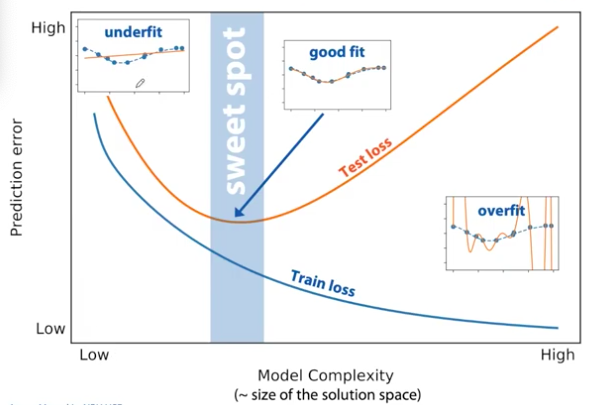
\includegraphics[scale=0.5]{traintest.png}
\end{figure}

The goal is to find the \textit{right level of limitations} - not too strict, not too loose.




\newpage
\section{Linear models}
\subsection{Linear models and linear regression}
\describesection{Linear models and examples. `Hidden power' of linear models via feature transformation. Examples of loss functions: MSE, MAE, MAPE and MSLE.}
\begin{framedef}
A \textit{linear model} is a model $\hat{f}(x)$ which is linear in its input (note this assumes a vector space structure on both the objects and targets). 
\end{framedef}

\begin{frameex}
Examples include:
\begin{itemize}
\item Linear regression, for example $\hat{f}(\vec{x}) = \pmb{\theta}^T \vec{x}$.
\item Classification, for example $\hat{f}(\vec{x}) = 1_{\{\pmb{\theta}^T\vec{x} > 0\}}$. This is non-linear as a function, but divides the target space by a line.
\end{itemize}
\end{frameex}

Linear models have a \textit{hidden power}. Problems which appear linearly inseparable (i.e. cannot be solved with linear models) can be made into problems which are tractable with linear models by \textit{transforming the features}. As an example, the data on the left below can be made linearly separable by introducing a new feature based on the sum of the squares of the coordinates of the points:

\begin{figure}[H]
\centering
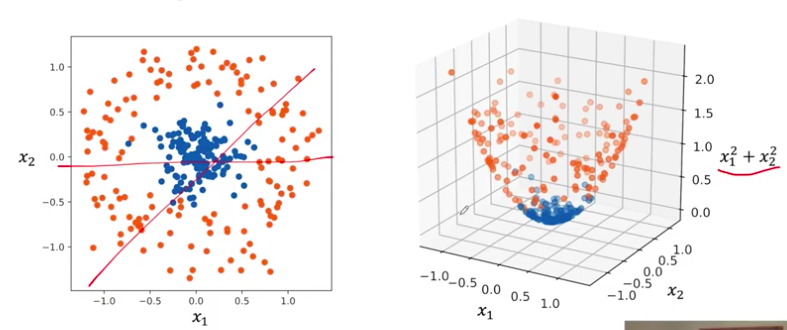
\includegraphics[scale=0.5]{hiddenlinear.png}
\end{figure}

Now a hyperplane separates the blue and orange sets.\\

In general, linear models motivate the construction of \textit{deep models}. Neural networks are just linear models with \textit{activation functions} between them (effecting some transformation). Thus better understanding linear models will help us understand deep neural networks. \\

We have already introduced linear regression as a linear model. Here, we update the notation:
\begin{framedef}
The \textit{model prediction} is $\hat{f}_{\pmb{\theta}}(\vec{x}) = \pmb{\theta}^T \vec{x}$, where $\pmb{\theta} \in \mathbb{R}^d$ is our \textit{parameter vector}, $\vec{x} \in \mathcal{X} \subseteq \mathbb{R}^d$ is our \textit{features vector}, and:
\begin{equation*}
\frac{1}{N} \sum_{i=1,...,N} \left( f(\vec{x}_i) - \hat{f}_{\pmb{\theta}}(\vec{x}_i) \right)^2
\end{equation*}
is our mean squared error loss, given a dataset. We wish to minimise this over $\pmb{\theta}$.
\end{framedef}


\newpage
Other loss functions are available. For example:
\begin{itemize}
\item \textbf{Mean absolute error (MAE).} This is given by:
\begin{equation*}
\frac{1}{N} \sum_{i=1,...,N} \left|f(\vec{x}_i) - \hat{f}_{\pmb{\theta}}(\vec{x}_i)\right|.
\end{equation*}
This grows linearly for large errors, rather than quadratically like mean squared error loss. In particular, it doesn't penalise large errors as much as mean squared error loss - it might be more suitable if there are outliers in your data which you do not wish to be biased against.
\item \textbf{Mean absolute percentage error (MAPE).} This is given by:
\begin{equation*}
\frac{1}{N} \sum_{i=1,..,N} \left| \frac{f(\vec{x}_i) - \hat{f}_{\pmb{\theta}}(\vec{x}_i)}{f(\vec{x}_i)} \right|.
\end{equation*} 
\item \textbf{Mean squared logarithmic error (MSLE).} This is given by:
\begin{equation*}
\frac{1}{N} \sum_{i=1,...,N} \left( \log(f(\vec{x}_i) + 1) - \log(\hat{f}_{\pmb{\theta}}(\vec{x}_i) + 1) \right)^2.
\end{equation*}
The $1$'s are there just to allow zero values of the targets. 
\end{itemize}
Both MAPE and MSLE provide a means of computing \textit{relative error}, so are useful when the targets span through a large range of magnitudes.\\

In general, applying different loss functions are also related to different assumptions about the data. A different loss function might be more suitable to a particular dataset.





\newpage
\subsection{Analytic solution}
\describesection{Analytic solution for linear models. Ill-conditioning and flat directions. Bias terms.}
Recall that earlier we defined the design matrix $X$, a matrix with rows given by the objects and columns given by the features. We can use this to rewrite the mean squared error loss as:
\begin{equation*}
\mathcal{L}_{\text{MSE}} = \frac{1}{N} \sum_{i=1,...,N} \left( f(\vec{x}_i) - \pmb{\theta}^T \vec{x}_i \right)^2 = \frac{1}{N} || \vec{y} - X \pmb{\theta} ||^2,
\end{equation*}
where $\vec{y} = (f(\vec{x}_1),...,f(\vec{x}_N))^T$.\\

To minimise this function, we can ignore the $1/N$ as it plays no role. Thus we wish to minimise $||\vec{y} - X\pmb{\theta}||^2$ over $\pmb{\theta}$. Analytically, the requirements are:
\begin{equation*}
\frac{\partial}{\partial \pmb{\theta}} \mathcal{L}_{\text{MSE}} = \vec{0}, \qquad \text{the matrix }\frac{\partial^2}{\partial \theta_i \partial \theta_j} \mathcal{L}_{\text{MSE}}\text{ of second derivatives should be positive definite.}
\end{equation*}
The first condition ensures we have an extremum, the second condition ensures that extremum is a minimum.

\begin{frameprop}
If the columns of $X$ are linearly independent, the solution to the above minimisation problem is $\pmb{\theta} = (X^TX)^{-1} \vec{y}$.\\

\textit{Proof:} Note that in general, the matrix $X^TX$ is always \textit{positive semi-definite}, since:
\begin{equation*}
\vec{v}^T X^T X\vec{v} = ||X\vec{v}||^2 \geq 0
\end{equation*}
for arbitrary $\vec{v}$. We see it is \textit{precisely} positive definite when the columns of $X$ are linearly independent (imagine the expression $X\vec{v}$ to be a linear combination of the columns of $X$). This additionally implies $X$ is invertible (e.g. all its eigenvalues are positive).\\

We can now consider the optimisation problem. The first derivative of $\mathcal{L}_{\text{MSE}}$ is easily computed:
\begin{equation*}
\frac{\partial}{\partial \pmb{\theta}} \mathcal{L}_{\text{MSE}} = \frac{1}{N}\frac{\partial}{\partial \pmb{\theta}} (\vec{y} - X \pmb{\theta})^T (\vec{y} - X\pmb{\theta}) = -\frac{2}{N}X^T (\vec{y} - X\pmb{\theta}) = \vec{0}.
\end{equation*}
This implies that $X^T \vec{y} - X^T X \pmb{\theta} = \vec{0}$. Since $X^TX$ is invertible, we can compute the solution:
\begin{equation*}
\pmb{\theta} = (X^T X)^{-1} X^T \vec{y}.
\end{equation*}
To check that this is a minimum, we must look at the second derivative. We find that the matrix of second derivatives is precisely:
\begin{equation*}
2X^TX.
\end{equation*}
In particular, this matrix is positive definite by the above. \qedsymbol
\end{frameprop}

In practice, there may be some linear dependence of the columns of $X$ (i.e. there may be some `feature correlations'). This affects the invertibility of the matrix $X^TX$ - we get \textit{flat directions}, and hence multiple solutions to the problem.

\begin{figure}[H]
\centering
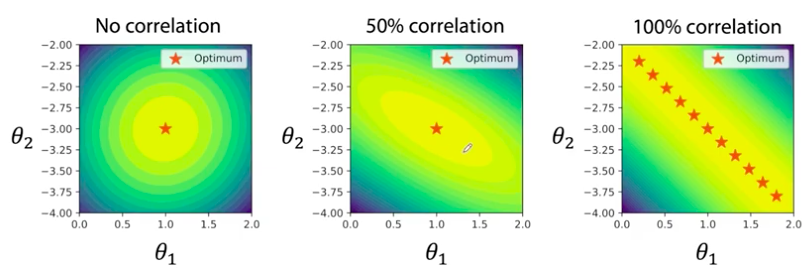
\includegraphics[scale=0.3]{featurecorrelations.png}
\end{figure}


\newpage
In the above we also assumed that our model took the form $\hat{f}_{\pmb{\theta}}(\vec{x}) = \pmb{\theta}^T \vec{x}$ for ease of calculation, but actually we can consider the more general linear model $\hat{f}_{\pmb{\theta}}(\vec{x}) = \pmb{\theta}^T \vec{x} + \theta_0$, where the term $\theta_0$ is called the \textit{bias term}. There is no need to redo any calculations here; we simply add a constant feature to the design matrix to account for this:
\begin{equation*}
X = \begin{pmatrix} x_1^1 & x_1^2 & \cdots & x_1^d \\ x_2^1 & x_2^2 & \cdots & x_2^d \\ \vdots & \vdots & \ddots & \vdots \\ x_N^1 & x_N^2 & \cdots & x_N^d \end{pmatrix} \qquad \rightarrow \qquad X =\begin{pmatrix} 1 & x_1^1 & x_1^2 & \cdots & x_1^d \\ 1 & x_2^1 & x_2^2 & \cdots & x_2^d \\ \vdots & \vdots & \vdots & \ddots & \vdots \\ 1 & x_N^1 & x_N^2 & \cdots & x_N^d \end{pmatrix}
\end{equation*}
Now when we multiply $X\pmb{\theta}$, one of the parameters will play the role of the bias term.

\begin{figure}[H]
\centering
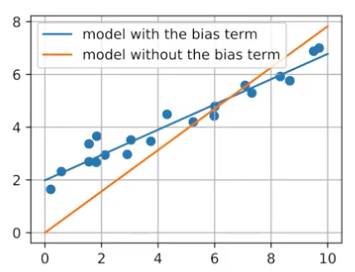
\includegraphics[scale=0.4]{biasterm.png}
\end{figure}





\newpage
\subsection{Numerical and stochastic optimisation: gradient descent}
\describesection{The gradient and its geometric interpretation. The gradient descent algorithm; convex functions. Overfitting and early stopping. Stochastic gradient descent.}
We have now discussed the analytic solution for the mean squared error loss minimisation problem in the context of a linear model. However, most loss functions do not allow an analytic solution, so it is important to discuss numerical solutions.\\

We being with some revision of the \textit{gradient}. Recall that the gradient of a scalar function on $\mathbb{R}^d$ is given by:
\begin{equation*}
\nabla f(\vec{x}) = \left( \frac{\partial f}{\partial x_1}(\vec{x}), ..., \frac{\partial f}{\partial x_d}(\vec{x}) \right).
\end{equation*}
The gradient always points in the \textit{direction of greatest increase} of the function. Hence if we start at a point, and move in the opposite direction to the gradient, we will get closer to a local minimum - this aids optimisation.\\

Let us formalise this:
\begin{framedef}
Given a smooth function $f : \mathbb{R}^d \rightarrow \mathbb{R}$ and an initial point $\vec{x}^{(0)}$, we define a recursive sequence of points via:
\begin{equation*}
\vec{x}^{(k)} = \vec{x}^{(k-1)} - \alpha \nabla f(\vec{x}^{(k-1)}),
\end{equation*}
where $\alpha \in \mathbb{R}_{> 0}$ is a constant called the \textit{learning rate}. This construction is called \textit{gradient descent iteration}.

\begin{figure}[H]
\centering
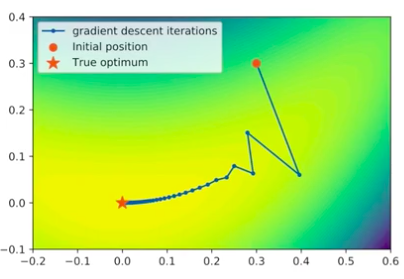
\includegraphics[scale=0.3]{gradientdescent.png}
\end{figure}
\end{framedef}

It is possible to show that:
\begin{frameprop}
For smooth, \textit{convex} functions with a single minimum $\vec{x}^* \in \mathbb{R}^d$, we have:
\begin{equation*}
f(\vec{x}^{(k)}) - f(\vec{x}^*) = O\left( \frac{1}{k} \right),
\end{equation*}
i.e. as we take more and more points, we approach the true minimum of the function.
\end{frameprop}

Gradient descent may also be applied to non-convex functions, but we may reach a minimum which is not \textit{global}, and the result may \textit{depend on the starting point}. 

\begin{figure}[H]
\centering
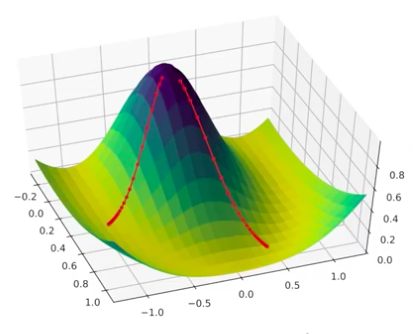
\includegraphics[scale=0.3]{nonconvex.png}
\end{figure}


\newpage
A useful property of gradient descent is that it can be used for \textit{regularisation} when our loss function is ill-defined; for example, when our $X^TX$ matrix above is not invertible (or not stably invertible). \\

In such cases, the true minimum typically has very large parameter values. These often correspond to \textit{overfitting}. To avoid this, we can start from a point where our initial parameters are \textit{small} and we can stop the gradient descent early (this is called \textit{early stopping}). This will typically be a better solution than the true minimum.

\begin{figure}[H]
\centering
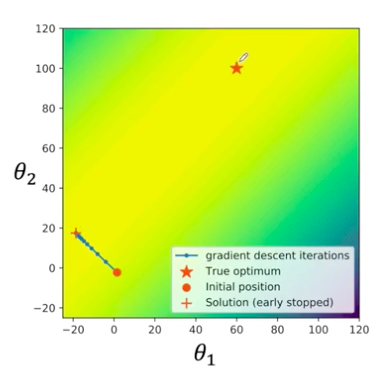
\includegraphics[scale=0.4]{regularisation.png}
\end{figure}

There is an important modification to the gradient descent algorithm called \textit{stochastic gradient descent}. Recall that in machine learning we typically optimise loss functions which are averages over some set of objects:
\begin{equation*}
L = \frac{1}{N} \sum_{i=1,...,N} \mathcal{L}\left(f(x_i), \hat{f}_{\theta}(x_i) \right).
\end{equation*}
For large $N$, gradient descent is computationally inefficient and may be unfeasible in terms of memory consumption. Stochastic gradient descent deals with this problem:
\begin{framedef}
Given a function $\hat{f}_{\pmb{\theta}} : \mathcal{X} \rightarrow \mathcal{Y}$ which depends on a parameter $\pmb{\theta} \in \mathbb{R}^d$, a starting point $\pmb{\theta}^{(0)}$, and a set of objects $x_1,...,x_N \in \mathcal{X}$, we define a recursive sequence of points as follows:
\begin{itemize}
\item At step $k$ of the process, pick some $l_k \in \{1,...,N\}$ at random.
\item Define:
\begin{equation*}
\pmb{\theta}^{(k)} = \pmb{\theta}^{(k-1)} - \alpha \nabla_{\pmb{\theta}} \mathcal{L}\left(f(x_{l_k}), \hat{f}_{\pmb{\theta}^{(k-1)}}(x_{l_k}) \right).
\end{equation*}
\end{itemize}
This is called \textit{stochastic gradient descent iteration}.
\end{framedef}

In the case of a smooth convex function, stochastic gradient descent also leads you to the unique minimum, but at a slower rate of $O(1/\sqrt{k})$ instead. This \textit{can} be improved by `batching' and other tricks.



\newpage
\subsection{Feature expansion}
\describesection{General description of feature transformation. Examples of polynomial feature transformations.}
Let us now see how linear models can be made more powerful by transforming their features.

\begin{framedef}
Given a design matrix $X$ of dimension $N \times d$, a \textit{feature transformation} via the function $\Phi : \mathbb{R}^d \rightarrow \mathbb{R}^{d'}$ is the induced map of the design matrix:
\begin{equation*}
X = \begin{pmatrix} x_1^1 & x_1^2 & \cdots & x_1^d \\ x_2^1 & x_2^2 & \cdots & x_2^d \\ \vdots & \vdots & \ddots & \vdots \\ x_N^1 & x_N^2 & \cdots & x_N^d \end{pmatrix} \qquad \rightarrow \qquad \Phi(X) =\begin{pmatrix} \Phi^1(x_1^1,...,x_1^d) & \cdots & \Phi^{d'}(x_1^1,...,x_1^d) \\ \Phi^1(x_2^1,...,x_2^d) & \cdots & \Phi^{d'}(x_2^1,...,x_2^d) \\ \vdots & \ddots & \vdots \\ \Phi^1(x_N^1,...,x_N^d) & \cdots & \Phi^{d'}(x_N^1,...,x_N^d)\end{pmatrix}
\end{equation*}
Finding good functions $\Phi$ to transform with is called \textit{feature engineering}. It is an important part of machine learning and requires a deep understanding of the underlying problem and the data.
\end{framedef}

\begin{frameex}
(\textbf{Polynomial features.}) Consider trying to fit the curve $y = x + \frac{1}{2}x^2$. This cannot be solved using only linear regression; a single line will not work.
\begin{figure}[H]
\centering
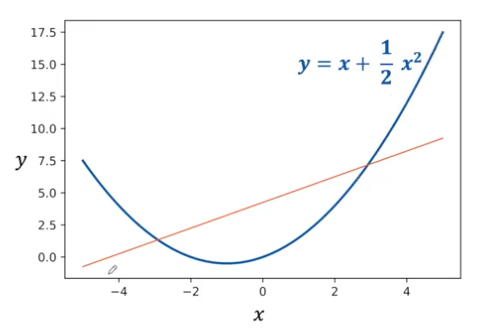
\includegraphics[scale=0.3]{quadvslinear.png}
\end{figure}
However, we can introduce a new feature via a feature transformation. Let $(x_1, x_2) = (x,x^2)$. Then in the new feature space, a linear estimate is really an estimate of the form $\hat{f}(\vec{x}) = \theta_1 x_1 + \theta_2 x_2 = \theta_1 x + \theta_2 x^2$, which facilitates fitting.
\begin{figure}[H]
\centering
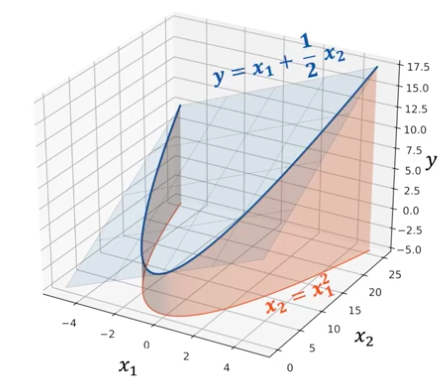
\includegraphics[scale=0.3]{featuretrans.png}
\end{figure}
\end{frameex}



\begin{frameex}
(\textbf{Polynomial features - general case}) Let $(x_i^1,x_i^2,...,x_i^d)$ be the original features of a dataset. We introduce as new features all unique multiplicative combinations of the form:
\begin{equation*}
(x_i^1)^{p_1}(x_i^2)^{p_2} ... (x_i^d)^{p_d},
\end{equation*}
where $p_1 + p_2 + \cdots + p_m \leq p$ (with $p$ the degree we expect to work).
\end{frameex}







\newpage
\section{Classification with linear models}

\subsection{Classification with linear regression}
\describesection{Classification problems; na\"{i}ve approach with MSE loss. Better approach with smooth approximations to $0$-$1$ loss.}
Consider a classification problem, with two classes, as shown below:
\begin{figure}[H]
\centering
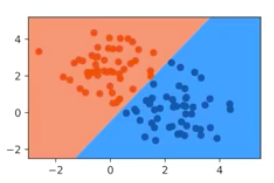
\includegraphics[scale=0.7]{classificationproblem.png}
\end{figure}
Since there are only two classes, we can assign numeric values to the classes - for our convenience, we choose $y = +1$ for one class (the `positive' class) and $y = -1$ for the other class (the `negative' class)\\

We can try to predict these targets with a linear model. To do so, we solve a linear regression problem using the model $\hat{y}_{\pmb{\theta}}(\vec{x}) = \pmb{\theta}^T\vec{x}$. To obtain the classified function, we then simply take the sign of the result:
\begin{equation*}
\hat{f}(\vec{x}) = \textrm{sign}(\hat{y}(\vec{x})).
\end{equation*}

This may seem like a reasonable approach, but you can face problems. Consider the following set:
\begin{figure}[H]
\centering
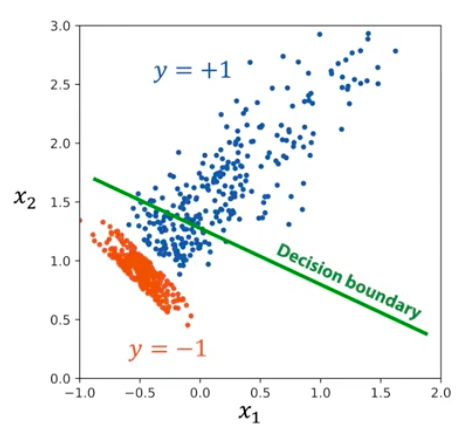
\includegraphics[scale=0.4]{decisionboundary.png}
\end{figure}
Here, the MSE loss makes the model avoid high errors, at the price of \textit{pushing the decision boundary} towards the class with higher spread.




\newpage

Therefore, we might try to use a different loss function. A good first example is \textit{$0$-$1$ loss}.
\begin{framedef}
For the above classification problem, we define the \textit{$0$-$1$ loss by}:
\begin{equation*}
\mathcal{L}_{0\text{-}1} = \frac{1}{N} \sum_{i=1,...,N} 1_{\{\pmb{\theta}^T \vec{x}_i y_i < 0\}}
\end{equation*}
where $y_i \in \{-1,+1\}$. We call $M = \pmb{\theta}^T \vec{x} y$ the \textit{margin}. When $M > 0$, we have a \textit{correct} classification, but when $M < 0$ we have an \textit{incorrect} classification. The higher the magnitude of $M$, the further an object is from the decision boundary. \\

The sum computes the number of times our linear regression misclassifies a point. 
\end{framedef}

Unfortunately, the resulting $0$-$1$ loss function is a piecewise constant function of $\pmb{\theta}$:
\begin{equation*}
\centering
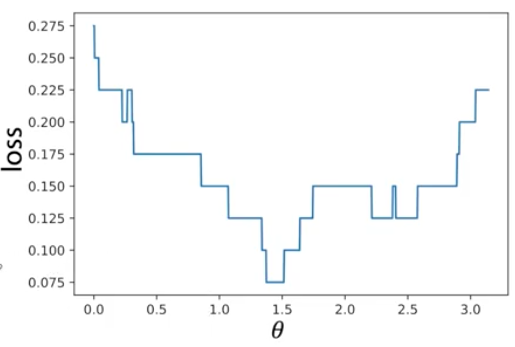
\includegraphics[scale=0.4]{01loss.png}
\end{equation*} 
This means that we cannot use \textit{gradient descent} to minimise our loss (of course, there are other methods - we will discuss them later).\\

Instead of using $0$-$1$ loss then, we could replace the sharp `step' function described by the loss by a \textit{differentiable upper bound}:
\begin{figure}[H]
\centering
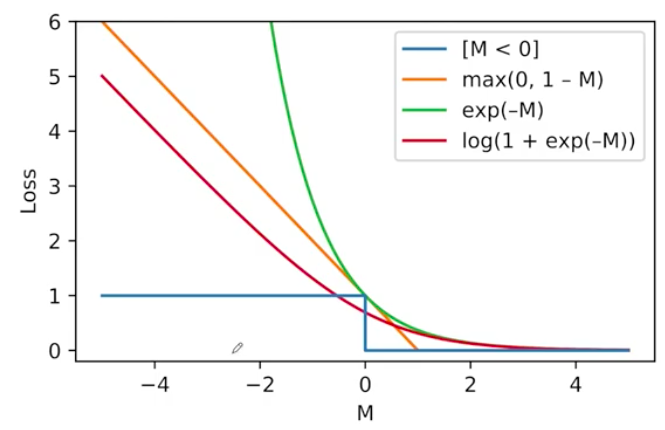
\includegraphics[scale=0.4]{upperbound.png}
\end{figure}
Examples are shown in the above figure (the red line can be scaled to be above the step function). We will discuss the red line (\textit{log loss}) in much more detail as we discuss \textit{logistic regression}.



\newpage
\subsection{Logistic regression}
\describesection{Logistic regression from class probabilities and maximum log likelihood. The sigmoid function and the logistic regression loss function.}
Let's depart from the discussion above, and approach things from a different way to start with. Consider modelling the \textit{class probabilities}: we introduce a function $\hat{f}_{\pmb{\theta}}(\vec{x})$ that gives the probability of an object $\vec{x}$ being in the class $y=+1$, so that:
\begin{equation*}
\mathbb{P}(y=+1 | \vec{x}) = \hat{f}_{\pmb{\theta}}(\vec{x}), \qquad \mathbb{P}(y=-1 | \vec{x}) = 1 - \hat{f}_{\pmb{\theta}}(\vec{x}).
\end{equation*}
How can we optimise such a model? We can fit with the \textit{maximum log likelihood}.\\

Recall that the \textit{likelihood} is defined by:
\begin{equation*}
\text{likelihood} = \prod_{i=1,...,N} \mathbb{P}(y_i|\vec{x}_i) = \prod_{i=1,...,N} \left( 1_{\{y_i = +1\}} \hat{f}_{\pmb{\theta}}(\vec{x}_i) + 1_{\{y_i = -1\}} \left(1 - \hat{f}_{\pmb{\theta}}(\vec{x}_i) \right) \right).
\end{equation*}
Maximising the logarithm likelihood allows us to obtain the best values of the parameter $\pmb{\theta}$:
\begin{equation*}
\pmb{\theta} = \underset{\pmb{\theta}}{\textrm{argmax}} \sum_{i=1,...,N} \left( 1_{\{y_i = +1\}} \log\left(\hat{f}_{\pmb{\theta}}(\vec{x}_i) \right) + 1_{\{y_i = -1\}} \log\left( 1 - \hat{f}_{\pmb{\theta}}(\vec{x}_i) \right) \right).
\end{equation*}
Note that the indicator functions can be moved out of the logarithm because only one of them is equal to $1$ at a time.\\

Once we have fitted the parameter values, we can for example predict the class the \textit{highest probability} for each $\vec{x} \in \mathcal{X}$ in the object space. More generally, we could not just choose the highest probability class but try to use a probability threshold that is suitable for our problem.


\minirule

Let's try to relate this back to linear models now. We need to ask: how can we map a linear model output to a probability value in $[0,1]$? A common choice is the \textit{sigmoid function}:
\begin{framedef}
The \textit{sigmoid function} is defined by:
\begin{equation*}
\sigma(x) = \frac{1}{1 + e^{-x}}.
\end{equation*}
It has the useful property that $1 - \sigma(x) = \sigma(-x)$. 
\end{framedef}
This can be applied to the above example, since we can define:
\begin{equation*}
\mathbb{P}(y=+1|\vec{x}) = \sigma(\pmb{\theta}^T \vec{x}). 
\end{equation*}
where $\pmb{\theta}^T \vec{x}$ is our linear model. The linear model $\pmb{\theta}^T \vec{x}$ then has the meaning of \textit{log odds ratio} between the two classes:
\begin{equation*}
\log\left( \frac{\mathbb{P}(y = +1 | \vec{x})}{\mathbb{P}(y = -1 | \vec{x})} \right) = \log\left( \frac{1}{1 + e^{-\pmb{\theta}^T \vec{x}}} \cdot \frac{1 + e^{-\pmb{\theta}^T \vec{x}}}{e^{-\pmb{\theta}^T \vec{x}}} \right) = \pmb{\theta}^T \vec{x}.
\end{equation*}
Therefore to bring everything together, we use the negative log likelihood as our loss function:
\begin{align*}
\mathcal{L} &= - \sum_{i=1,...,N} \left( 1_{\{y_i = +1\}} \log\left(\hat{f}_{\pmb{\theta}}(\vec{x}_i) \right) + 1_{\{y_i = -1\}} \log\left( 1 - \hat{f}_{\pmb{\theta}}(\vec{x}_i) \right) \right) \\[1.5ex]
&= \sum_{i=1,...,N} \left( 1_{\{y_i = +1\}} \log\left(\sigma(\pmb{\theta}^T \vec{x}_i)\right) + 1_{\{y_i = -1\}} \log\left(  \sigma(-\pmb{\theta}^T \vec{x}_i) \right) \right)\\[1.5ex]
&= - \sum_{i=1,...N} \log\left( \sigma(\pmb{\theta}^T \vec{x}_i y_i ) \right) = \sum_{i=1,...N} \log\left(1 + e^{-\pmb{\theta}^T \vec{x}_i y_i} \right).
\end{align*}
This is the same as the `red' example we used above when we discussed upper bounds on $0$-$1$ loss. We can apply gradient descent or stochastic gradient descent here.


\newpage
Applying to the dataset above, the decision boundary is in the correct place with logistic regression:
\begin{figure}[H]
\centering
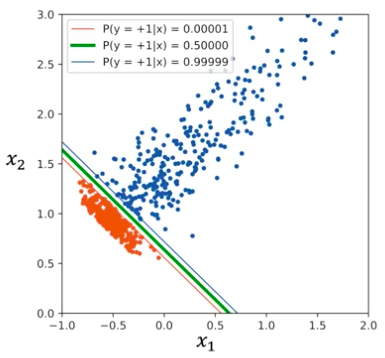
\includegraphics[scale=0.4]{decisionboundary2.png}
\end{figure}
Note that when the classes are linearly separable as above, for any correct decision boundary, mapping $\pmb{\theta} \rightarrow C \cdot \pmb{\theta}$ for some $C > 1$ keeps the boundary at the same place, yet improves the loss. The ideal fit is when the sigmoid turns into a step function (at infinitely large $\pmb{\theta}$.\\

If the classes overlap however, the predicted class probability changes smooth, and the loss has a finite minimum.

\begin{figure}[H]
\centering
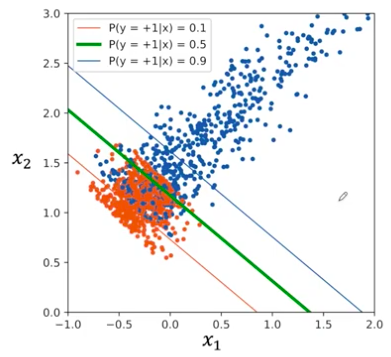
\includegraphics[scale=0.4]{decisionboundary3.png}
\end{figure}



\newpage
\subsection{Multinomial logistic regression}
\describesection{Logistic regression for many classes using class probabilities; symmetry of the parameters. The multinomial logistic regression loss function.}
Similarly to the binary case, we can model the class probabilities when there are more classes than $2$. Let's model the \textit{unnormalised} class probabilities as:
\begin{equation*}
\tilde{\mathbb{P}}(y = k | \vec{x}) = \exp\left( \pmb{\theta}_k^T \vec{x} \right),
\end{equation*}
where we now have $K$ parameter vectors, $k = 1,...,K$. The normalised probabilities can be straightforwardly obtained:
\begin{equation*}
\mathbb{P}(y = k | \vec{x}) = \frac{\exp\left( \pmb{\theta}_k^T \vec{x} \right)}{\sum_{k'=1,...,K} \exp(\pmb{\theta}_{k'}^T \vec{x})}
\end{equation*}
This function is called \textit{softmax} and is commonly used in neural networks.\\

Note that there is a transformational symmetry here: transforming $\pmb{\theta}_k \mapsto \pmb{\theta}_k + \vec{v}$ by some constant vector $\vec{v}$ does not affect the normalised probability. We have:
\begin{equation*}
\tilde{\mathbb{P}}(y = k | \vec{x}) = e^{\pmb{\theta}_k^T\vec{x}} \rightarrow e^{\vec{v}^T \vec{x}} \cdot e^{\pmb{\theta}_k^T \vec{x}} = e^{\vec{v}^T \vec{x}} \cdot \tilde{\mathbb{P}}(y = k | \vec{x}).
\end{equation*}
The remaining exponential cancels out in the ratio in the normalised probabilities. Therefore, we have some extra degree of freedom, which we are free to choose - we can therefore set $\pmb{\theta}_K = \vec{0}$ without loss of generality for example (i.e. we set the last parameter to zero). We are left with $K-1$ parameter vectors.\\

Individual linear outputs $\pmb{\theta}_k^T \vec{x}$ now have the meaning of \textit{log odds ratio} between the classes $k$ and $K$:
\begin{equation*}
\log\left( \frac{\mathbb{P}(y = k | \vec{x})}{\mathbb{P}(y = K | \vec{x})} \right) = \log\left( \frac{\tilde{\mathbb{P}}(y = k | \vec{x})}{\tilde{\mathbb{P}}(y = K | \vec{x})} \right) = \log\left( \frac{e^{\pmb{\theta}_k^T \vec{x}}}{e^0} \right) = \pmb{\theta}_k^T \vec{x}.
\end{equation*}
Putting everything into the negative log likelihood function, we again get our loss function:
\begin{equation*}
\mathcal{L} = - \sum_{i=1,...,N} \log\left( \frac{\exp(\pmb{\theta}_{y_i}^T \vec{x}_i)}{1 + \sum_{k' = 1,...,K-1} \exp\left( \pmb{\theta}_{k'}^T \vec{x}_i \right)}\right),
\end{equation*}
where $\pmb{\theta}_K = \vec{0}$. Again, this can be optimised \textit{numerically} using gradient descent or stochastic gradient descent.


\newpage
\subsection{Multiclass classification: general approach}
\describesection{One-versus-rest multiclass classification. Comparison with logistic regression.}
In fact, you are not limited to use logistic regression for multiclass classification - you are able to use any linear model.\\

For a problem with $K$ classes, introduce $K$ predictors:
\begin{equation*}
\hat{f}_k(\vec{x}) : \mathcal{X} \rightarrow \mathbb{R}
\end{equation*}
for $k = 1,..., K$ each of which outputs a corresponding \textit{class score}. We can use this to predict the class with the \textit{highest score}:
\begin{equation*}
\hat{y}_i = \underset{k}{\textrm{argmax}} \hat{f}_k(\vec{x}_i).
\end{equation*}
For example, any binary linear classification model can be converted to a multiclass classification with the \textit{one-versus-rest} strategy:
\begin{itemize}
\item For each class $k$ train a binary model $\hat{f}_k(\vec{x}) = \pmb{\theta}^T_{(k)}\vec{x}$ separating the given class from all others, $\hat{y}^{\text{one-vs-rest}}_{(k)} = \textrm{sign}(\hat{f}_k(\vec{x}))$. 
\item Use the outputs of $\hat{f}_k$ as class scores for multiclass classification:
\begin{equation*}
\hat{y}_i = \underset{k}{\textrm{argmax}} \hat{f}_k(\vec{x}_i).
\end{equation*}
\end{itemize}

\begin{frameex}
In the following three-class classification, the one-versus-rest splits given by using the appropriate binary classifiers are shown below:
\begin{figure}[H]
\centering
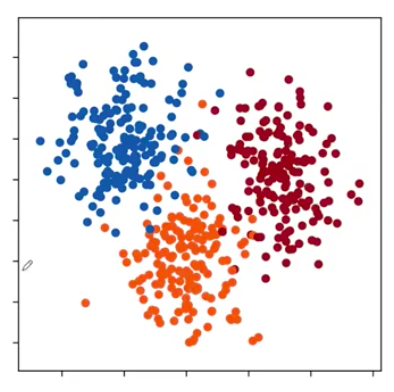
\includegraphics[scale=0.4]{onevsrest1.png}
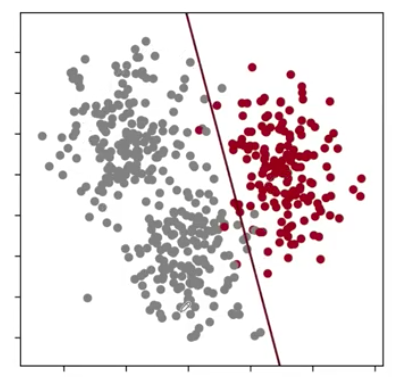
\includegraphics[scale=0.4]{onevsrest2.png}
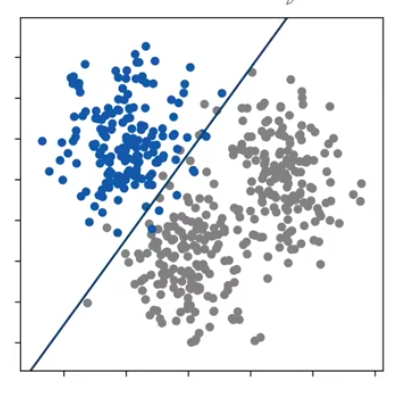
\includegraphics[scale=0.4]{onevsrest3.png}
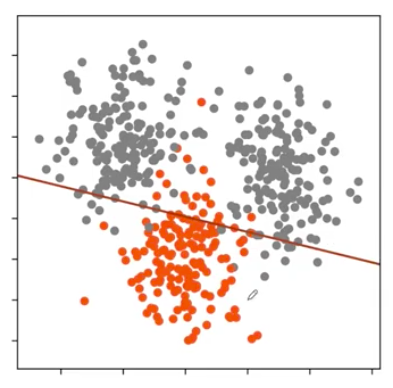
\includegraphics[scale=0.4]{onevsrest4.png}
\end{figure}

\newpage
The resulting decision boundaries can be built up as follows:
\begin{figure}[H]
\centering
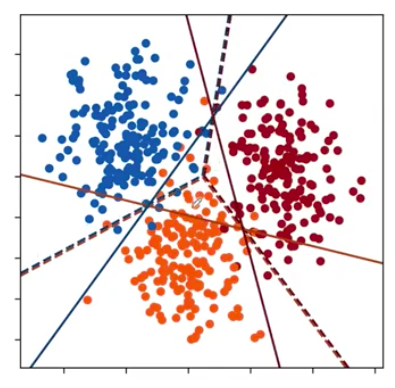
\includegraphics[scale=0.4]{decisionboundaries2.png}
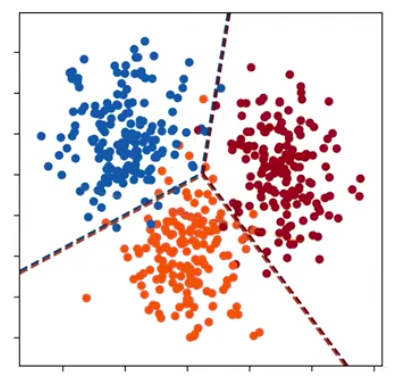
\includegraphics[scale=0.4]{decisionboundaries3.png}
\end{figure}
\end{frameex}

Is the one-vs-rest approach better than multinomial logistic regression however? Some problems are not linearly separable, so one-vs-rest results in biased class probabilities whilst logistic regression is still quite accurate:
\begin{figure}[H]
\centering
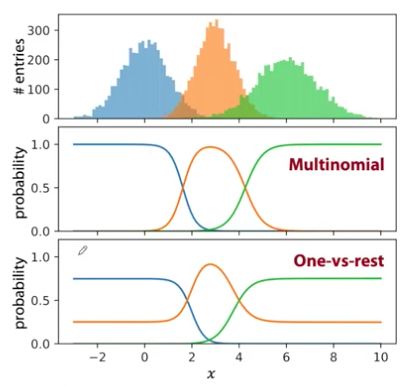
\includegraphics[scale=0.6]{logisticvsonevsrest.png}
\end{figure}





\newpage
\section{Model regularisation}

\subsection{The problem of overfitting}
\describesection{Recap of overfitting and test set.}
Overfitting is the tendency of a model to adjust to random fluctuations in the data. This can be detected by a model making poor predictions on the \textit{test set}.

\begin{figure}[H]
\centering
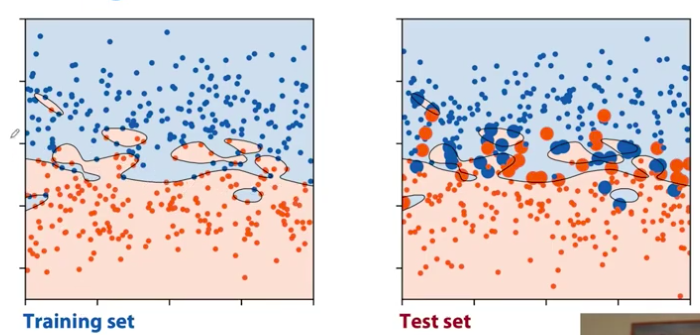
\includegraphics[scale=0.4]{overfitting.png}
\end{figure}

Recall that we need to use a model complexity such that we don't underfit, and we don't overfit - we need to find the `sweet spot' in between.

\minirule

\subsection{Prediction error decomposition}
\describesection{Decomposition of error sources: model variance, bias, and irreducible error. The bias-variance tradeoff. Bias and variance of linear models.}
Before talking about regularisation, let's discuss the prediction error of a model. Assume that there's the following unknown relation between features and targets:
\begin{equation*}
y = f(x) + \epsilon,
\end{equation*}
where $\epsilon$ is some random noise, $\mathbb{E}[\epsilon] = 0$ and $\textrm{Var}[\epsilon] = \sigma_{\epsilon}^2$. Let's denote a training set as $\tau$. We want to study the \textit{expected squared error} for the model $\hat{f}_{\tau}$ trained on the dataset $\tau$:
\begin{equation*}
\textrm{exp.sq.err}(x) = \underset{\tau, y}{\mathbb{E}}\left[ (\hat{f}_{\tau}(x) - y )^2 | x \right].
\end{equation*}
The target $y$ is sampled independently of the training set.\\

We can rewrite this expression in the following form, by adding and subtracting the `prediction of the expected model' and the `ground truth' $f(x)$ (without the noise):
\begin{align*}
\textrm{exp.sq.err}(x) &= \underset{\tau, y}{\mathbb{E}}\left[ (\hat{f}_{\tau}(x) - y )^2 | x \right]\\[1.5ex]
&= \underset{\tau,y}{\mathbb{E}}\left[ \left( (\hat{f}_{\tau}(x) - \underset{\tau'}{\mathbb{E}}[\hat{f}_{\tau'}(x)]) + (\underset{\tau'}{\mathbb{E}}[\hat{f}_{\tau'}(x)] - f(x)]) + (f(x) - y)\right)^2 \bigg| x\right]\\[1.5ex]
&= \underset{\tau}{\mathbb{E}}\left[ \left(\hat{f}_{\tau}(x) - \underset{\tau'}{\mathbb{E}}[\hat{f}_{\tau'}(x)] \right)^2\right] + \left( \underset{\tau'}{\mathbb{E}}[\hat{f}_{\tau'}(x)] - f(x) \right)^2 + \underset{y}{\mathbb{E}}[(f(x) - y)^2 | x].
\end{align*}
In the final step, we have expanded everything and used the fact that the cross-term expectation are $0$ (this follows from the fact that $\tau, y$ are sampled independently).


\newpage
\noindent The remaining terms have important interpretations:
\begin{itemize}
\item The first term is the \textit{variance of the model}. It quantifies how `unstable' the model is with respect to the noise in the training data.
\item The second term is the \textit{squared bias}. It is how much the `expected model' differs from the ground truth.
\item The third term is the \textit{irreducible error}. Substituting the true dependence $y$, we find it is just given by $\sigma_{\epsilon}^2$. This error cannot be eliminated.
\end{itemize}
The first two errors on the other hand, can be removed by changing the model. Typically there's a \textit{tradeoff} between the two types of errors:
\begin{figure}[H]
\centering
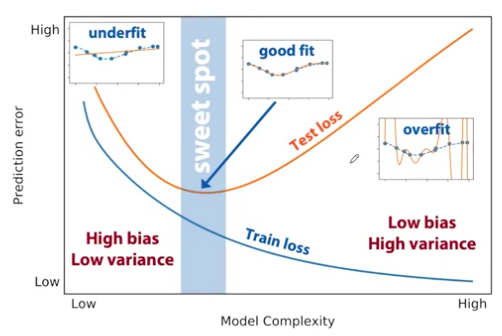
\includegraphics[scale=0.4]{biasvariancetradeoff.png}
\end{figure}
For low model complexity, the \textit{bias} is high because we are artificially simplifying the model - it doesn't depend much on the data (it has `low variance'). The opposite is true for high model complexity. This tradeoff is called the \textit{bias-variance tradeoff}.

\begin{frameex}
Let's compute the bias and variance of a linear model. For each expectation $\mathbb{E}$ with respect to $\tau$, we will assume that the features are \textit{fixed}, i.e. $X_{\tau} = X$ (i.e. the design matrix is constant), and only the target vector $y_{\tau}$ is random. This simplification allows us to analytically compute the result.\\

Recall the solution for the linear regression model with the MSE loss:
\begin{equation*}
\hat{f}_{\tau}(\vec{x}) = \pmb{\theta}_{\tau}^T\vec{x}, \qquad \pmb{\theta}_{\tau} = (X^TX)^{-1} X^T \pmb{y}_{\tau}.
\end{equation*}
The \textit{bias term} from the above error decomposition is:
\begin{equation*}
\textrm{bias}(\vec{x}) = \underset{\tau}{\mathbb{E}}[\hat{f}_{\tau}(\vec{x})] - f(\vec{x}) = \underset{\tau}{\mathbb{E}}\left[ \vec{x}^T (X^TX)^{-1}X^T \vec{y}_{\tau} \right] - \vec{x}^T \pmb{\theta}_{\text{true}}
\end{equation*}
We also assume that the true dependence is indeed linear, i.e. $f(\vec{x}) = \vec{x}^T \pmb{\theta}_{\text{true}}$ for some $\pmb{\theta}_{\text{true}}$.\\

Since $X$ does not depend on the sampling dataset $\tau$, we can move lots of things out of the expectation, leaving:
\begin{equation*}
\vec{x}^T (X^TX)^{-1}X^T \underset{\tau}{\mathbb{E}}[\vec{y}_{\tau} - \vec{x}^T \pmb{\theta}_{\text{true}} = \vec{x}^T (X^TX)^{-1} X^TX \pmb{\theta}_{\text{true}} - \vec{x}^T \pmb{\theta}_{\text{true}} = \vec{x}^T \pmb{\theta}_{\text{true}} - \vec{x}^T \pmb{\theta}_{\text{true}} = 0.
\end{equation*}
Hence we see that the linear regression model is \textit{unbiased}, provided the true dependence is linear.


\newpage
Now let's consider the \textit{variance term}:
\begin{equation*}
\textrm{variance}(\vec{x}) = \underset{\tau}{\mathbb{E}} \left[ \left(\hat{f}_{\tau}(\vec{x}) - \underset{\tau'}{\mathbb{E}}[\hat{f}_{\tau'}(\vec{x})]\right)^2 \right].
\end{equation*}
It can be shown that:
\begin{equation*}
\textrm{variance}(\vec{x}) = \sigma_{\epsilon}^2 \vec{x}^T (X^TX)^{-1} \vec{x},
\end{equation*}
so that the variance error component is a \textit{quadratic form}, defined by the $(X^TX)^{-1}$ matrix. We can diagonalise $X^TX$ giving:
\begin{equation*}
\textrm{variance}(\vec{x}) = \sigma_{\epsilon}^2 \tilde{\vec{x}}^T \Lambda^{-1} \tilde{\vec{x}},
\end{equation*}
where $\Lambda = \textrm{diag}\{\lambda_1,...,\lambda_d\}$ is the diagonal matrix of eigenvalues of $X^TX$. This means that \textit{small eigenvalues amplify the model variance}. This happens when $X^TX$ is ill-defined, e.g. when the features are correlated.

\begin{figure}[H]
\centering
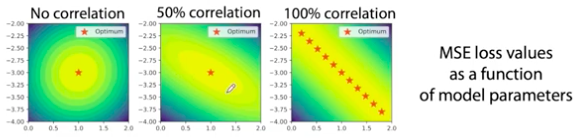
\includegraphics[scale=0.4]{linearvariance.png}
\end{figure}
\end{frameex}

In a high variance model, we expect that a small perturbation data will lead to a large change in the prediction.


\minirule


\subsection{Regularisation}
\describesection{Regularisation methods: $L2$ regularisation, $L1$ regularisation, and elastic net regression. Comparison of methods; sparsity vs weight-sharing.}
How can we reduce the variance of a model? If only we could \textit{increase the eigenvalues} of the matrix $X^TX$. In fact, we can do this manually:
\begin{equation*}
X^TX \rightarrow X^TX + \alpha I,
\end{equation*}
for $\alpha > 0$, with $I$ a unit $d \times d$ matrix. This is called \textit{$L2$ regularisation}.\\

In this case, we change the solution to:
\begin{equation*}
\hat{f}_{\tau}(\vec{x}) = \vec{x}^T (X^TX + \alpha I)^{-1} X^T \vec{y}_{\tau}.
\end{equation*}
Now the model is \textit{no longer biased}. We \textit{increased bias to reduce variance} (we no longer get zero for the bias term of this model.
\begin{figure}[H]
\centering
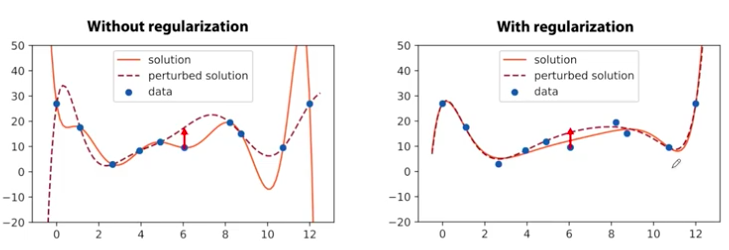
\includegraphics[scale=0.4]{L2regularisation.png}
\end{figure}



\newpage
By regularising the model, we increase the training loss and decrease the test loss. This improves the \textit{generalisability} of the model.

\begin{figure}[H]
\centering
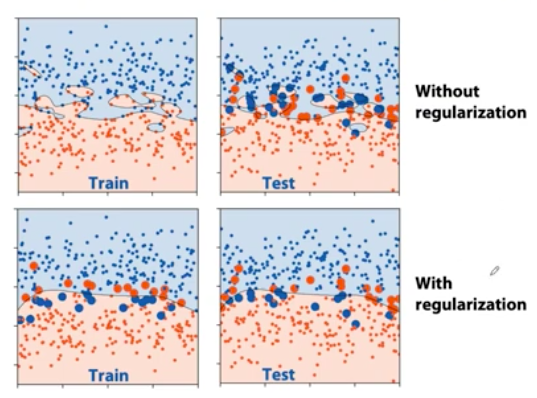
\includegraphics[scale=0.4]{generalisability.png}
\end{figure}

In order to understand this trick better, let's reverse engineer the loss function it optimises. We have the solution $\hat{f}_{\tau}(\vec{x}) = \vec{x}^T (X^T X + \alpha I)^{-1} X^T \vec{y}_{\tau}$, so the $\pmb{\theta}_{\tau}$ vector should be given by:
\begin{equation*}
\pmb{\theta}_{\tau} = (X^TX + \alpha I)^{-1} X^T \pmb{y}_{\tau}.
\end{equation*}
Regrouping the terms, we have:
\begin{equation*}
(XT^X + \alpha I)\pmb{\theta}_{\tau} = X^T \pmb{y}_{\tau} \qquad \Rightarrow \qquad X^T (X\pmb{\theta}_{\tau} - \vec{y}_{\tau}) + \alpha \pmb{\theta}_{\tau} = \vec{0}.
\end{equation*}
In fact, this is the equation $\partial \mathcal{L} / \partial \pmb{\theta}_{\tau} = \vec{0}$ for the loss function:
\begin{equation*}
\mathcal{L} = ||X\pmb{\theta}_{\tau} - \vec{y}_{\tau}||^2 + \alpha || \pmb{\theta}_{\tau}||^2.
\end{equation*}
This explains the origin of the term \textit{$L2$ regularisation}. The model minimises the MSE loss with an \textit{$L2$ penalty theorem} (this model is also called \textit{ridge regression}).\\

There are other similar regularisation methods:
\begin{itemize}
\item \textit{$L2$ regularisation} or \textit{ridge regression} takes as the loss function $\mathcal{L} = ||X \pmb{\theta}_{\tau} - \vec{y}_{\tau}||^2 + \alpha || \pmb{\theta}_{\tau}||^2$.
\item \textit{$L1$ regularisation} or \textit{lasso regularisation} takes as the loss function $\mathcal{L} = ||X \pmb{\theta}_{\tau} - \vec{y}_{\tau}||^2 + \alpha||\pmb{\theta}_{\tau}||_1$ (where $|| \cdot ||_1$ denotes the $L1$ norm.
\item \textit{Elastic net regression} is a combination of the two:
\begin{equation*}
\mathcal{L} = ||X\pmb{\theta}_{\tau} - \vec{y}_{\tau}||^2 + \alpha || \pmb{\theta}_{\tau}||^2 + \beta || \pmb{\theta}_{\tau}||_{1}.
\end{equation*}
\end{itemize}

The introduction of regularisation methods drive the parameters towards smaller values, yet they \textit{induce different properties} of the solution.

\begin{figure}[H]
\centering
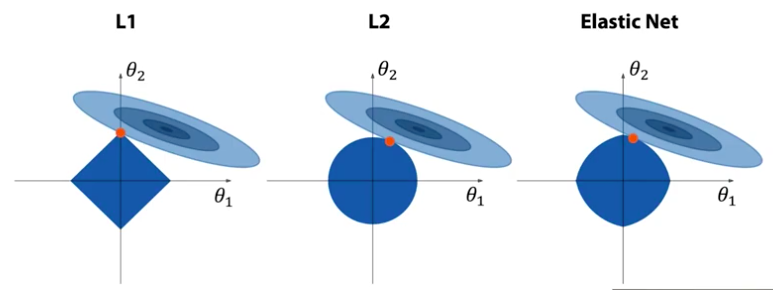
\includegraphics[scale=0.4]{diffregularisations.png}
\end{figure}


\newpage
For example, the $L1$ regularisation term has unit ball given by a diamond in $\theta_1, \theta_2$ space (i.e. the surface where $||\pmb{\theta}||_{1} = 1$). It's quite likely that among all the points at the perimeter of the diamond (where the penalty term does not change), the intersection is most likely at the coordinate axes. This means that this loss tends to \textit{sparsify the solution} - it tends to set some parameters to zero.\\

For the $L2$ regularisation, we instead have \textit{weight sharing} - it uniformly drags the values of the parameters towards zero.\\

The elastic net is a compromise between the two approaches.


\minirule

\subsection{Probabilistic view}
\describesection{Relationship of regularisation to probabilities and maximum likelihood.}
Let's revisit our assumption about the data, $y = f(x) + \epsilon$. Let's now assume that the label noise is \textit{normally distributed}, $\epsilon \sim \mathcal{N}(0,\sigma_{\epsilon}^2)$. This means that the targets, given the objects, are also normally distributed:
\begin{equation*}
y|x \sim \mathcal{N}(f(x), \sigma_{\epsilon}^2).
\end{equation*}
We want our model $\hat{f}_{\theta}(x)$ to fit the true dependence $f(x)$, i.e. we define a \textit{probabilistic model}:
\begin{equation*}
y|x \sim \mathcal{N}(\hat{f}_{\theta}(x),\sigma_{\epsilon}^2),
\end{equation*}
where the mean of the normal distribution is described by our function.\\

Our model can be fitted with the maximum likelihood approach:
\begin{equation*}
L = \prod_{i=1,...,N} \mathcal{N}(y_i | \hat{f}_{\theta}(x_i), \sigma_{\epsilon}^2).
\end{equation*}
Maximising this with respect to $\theta$ is equivalent to minimising the negative log likelihood,
\begin{gather*}
-\log(L) = \sum_{i=1,...,N} \log(\mathcal{N}(y_i | \hat{f}_{\theta}(x_i), \sigma_{\epsilon}^2)) = - \sum_{i=1,...,N} \left[ \log\left( \exp\left( - \frac{(y_i - \hat{f}_{\theta}(x_i) )^2}{2 \sigma_{\epsilon}^2} \right) \right) - \log(\sqrt{2 \pi} \sigma_{\epsilon}^2) \right] \\[1.5ex]
= C \cdot \sum_{i=1,...,N} (y_i - \hat{f}_{\theta}(x_i))^2 + \text{constant}.
\end{gather*}
Thus we just get MSE loss! Thus MSE loss is equivalent to modelling the probability with a normal label noise.\\

You can do similar tricks for other loss functions and show that different probabilistic models lead to different loss functions.


\minirule

\subsection{Bayesian view}
\describesection{Relationship of regularisation to Bayesian priors.}
In the Bayesian view, we treat both data $(X,y)$ and model parameters ($\theta$) as random variables. We estimate the parameter distribution given the observed data via Bayes' rule:
\begin{equation*}
p(\theta | X,y) = \frac{p(y | \theta,X) p(\theta)}{\displaystyle \int \left( p(y | \theta,X) p(\theta) \right) \ d\theta}
\end{equation*}
We assume that $\theta, X$ are independent variables here. Here, $p(\theta)$ is our prior knowledge about the model parameters (our belief about how they are distributed before we see any data). The function $p(y | \theta, X)$ is our likelihood function. The distribution $p(\theta | X,y)$ is called the \textit{posterior distribution}, and is our knowledge about the model after seeing data. The denominator is called `evidence' (the probability of observing the data when the parameter uncertainty is integrated out). \\

To get some estimate of the parameter, we can calculate the \textit{maximum a posteriori} (where we ignore the denominator since is it is integrated over $\theta$ - the maximum is the same as the maximum of the numerator):
\begin{equation*}
\hat{\theta} = \underset{\theta}{\textrm{argmax}}\ p(y | \theta, X) p(\theta) = \underset{\theta}{\textrm{argmin}}\left[ - \log(p(y | \theta, X) - \log(p(\theta)) \right]
\end{equation*}
Similarly, the maximum is the same as the minimum negative log likelihood. The term $\log(p(\theta))$ is called a \textit{regularising} term.

\begin{frameex}
Suppose we model the data with a normal distribution $y|x \sim \mathcal{N}(\hat{f}_{\theta}(x), \sigma_{\epsilon}^2)$. Suppose the prior is normal too $\theta \sim \mathcal{N}(0, \sigma_{\theta}^2 I)$, where $I$ is the unit matrix so that the parameters are uncorrelated. Then maximum a posteriori estimate corresponds to minimising the following loss:
\begin{equation*}
\mathcal{L} = -\log(p(y|\theta,X)) - \log(p(\theta)) = C_1 \sum_{i=1,...,N} (\hat{f}_{\theta}(x_i) - y_i)^2 + C_2 || \theta||^2 + \text{constant}.
\end{equation*}
In other words a normal prior is equivalent to $L2$ regularisation of the parameters.
\end{frameex} 

Choosing different priors will lead to different regularisation of the parameters.





\end{document}
